\documentclass{hw}
\hwname{6 / Radicals / Notes C2}

\begin{document}

\section*{Class 2}

\subsection*{\normalsize HW / Review}
\begin{itemize}
    \item 
    \begin{align*}
        -\sqrt{225} &= -\sqrt{9 \times 25} \\
                    &= -3 \cdot 5 \\
                    &= 15
    \end{align*}
    \item 
    \begin{align*}
        -\sqrt{\frac{5}{72}} &= -\sqrt{\frac{5}{36 \cdot 2}} \\
                             &= -\frac{\sqrt{5}}{6 \sqrt{2}}
    \end{align*}
    \item 
    \begin{align*}
        -\sqrt[4]{\frac{1}{16}} &= -\frac{1}{2}
    \end{align*}
    \item 
    \begin{align*}
        -\sqrt[3]{0.001} &= -\sqrt[3]{0.01 \times 0.01 \times 0.01} \\
                         &= -0.1
    \end{align*}
    \item 
    \begin{align*}
        -2x\sqrt{3} \cdot 5x\sqrt{27} &= 10x \cdot \sqrt{3} \cdot \sqrt{9 \cdot 3} \\
                                      &= 10x \cdot \sqrt{3} \cdot 3 \sqrt{3} \\
                                      &= 90x^2
    \end{align*}
    \item 
    \begin{align*}
        -2\sqrt{3x} \cdot 3\sqrt{6x} &= 6\sqrt{18x^2} \\
                                     &= 6\sqrt{9 \cdot 2x^2} \\
                                     &= 6 \cdot 3x \sqrt{2} \\
                                     &= 18x \sqrt{2}
    \end{align*}
    \item \( -\sqrt{a^2} = a \)
    \item \( -\sqrt{a^4} = a^2 \)
    \item \( -\sqrt[3]{a^6} = a^2 \)
\end{itemize}

\subsection*{\normalsize Simplest Radical Form}
It was is useful to have tables of square roots, especially for low natural numbers. \\
Noone likes division - especially when the divisor is a complicated number. \\
The simplest radical form is very useful in actual calculations (before calculators and computers).

{\centering
\fbox{
\parbox{\dimexpr\linewidth-2\fboxsep-2\fboxrule\relax}{
Rules for Simplest Radical Form:
\begin{itemize}
    \item No radicand contains a factor that’s a perfect $n$-th power.
    \item Every denominator has been rationalized.
    \begin{itemize}
        \item No radicand is a fraction.
        \item No radical is in the denominator.
    \end{itemize}
\end{itemize}
}}
\par}

\begin{minipage}{0.5\textwidth}
\centering
    \begin{align*}
        -\sqrt{\frac{5}{3}} &= \sqrt{\frac{5}{3} \cdot 3} \\
                            &= \sqrt{\frac{15}{9}} \\
                            &= \frac{\sqrt{15}}{3}
    \end{align*}
\end{minipage}
\begin{minipage}{0.5\textwidth}
\centering
    \begin{align*}
        -\frac{4}{\sqrt[3]{c}} &= \frac{4}{\sqrt[3]{c}} \cdot \frac{\sqrt[3]{c^2}}{\sqrt[3]{c^2}} \\
                               &= \frac{4 \sqrt[3]{c^2}}{\sqrt[3]{c^3}} \\
                               &= \frac{4 \sqrt[3]{c^2}}{c}
    \end{align*}
\end{minipage}

\subsection*{\normalsize Inverse functions}
Examples - Add and Subtract, Multiply and Divide. \\
Similarly, "Squaring" and "Taking the square-root" are Inverse functions of each other.

\newpage
\subsection*{\normalsize Gravitation Force problem}
Some laws of nature have squares - especially for the distance terms.

\subsubsection*{\normalsize Problem Statement}

\begin{figure}[h]
    \centering
    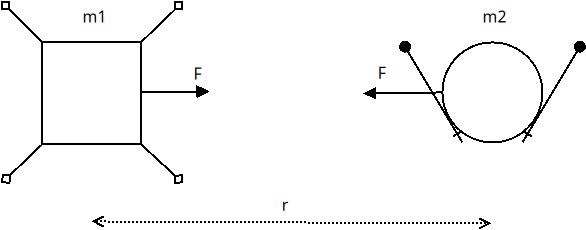
\includegraphics[width=0.9\textwidth]{dia/radicals-satellites.png}
    \caption{Two satellites in space.}
    \label{fig:satellites}
\end{figure}

Two space satellites, each with a mass of 100 kg, are observed to attract each other with a gravitational force of 25 Newtons.\\
The force follows the equation:

{\centering
$F = G \frac{m_1 m_2}{r^2}$
\par}

where,
\begin{itemize}
    \item $m_1$ and $m_2$ are the masses of the two objects in kilograms
    \item $r$ is the distance between the objects in meters
    \item $G$, the gravitational constant, is equal to 1 (in this simplified universe)
    \item $F$ is the gravitational force between the two objects in Newtons 
\end{itemize}
\bigskip
What is the distance between the two satellites?

\subsubsection*{\normalsize Solution}
\begin{align*}
25 &= \frac{1 \times 100 \times 100}{r^2} \\
r^2 &= \frac{10000}{25} \\
r^2 &= 400 \\
r &= 20
\end{align*}
The distance between the two satellites is 20 meters.

\end{document}